\section{Background}
\label{sec:background}

Docker~\cite{docker} is a popular virtualization technology
that extends traditional OS containers with higher level
functionalities.
%
It allows to efficiently package an application and its runtime dependencies
in a container image to simplify and automate application deployment~\cite{slacker}.
%
%It automates the deployment of software and allows to efficiently package an
%application with its runtime dependencies in a container image~\cite{slacker}.
%


\begin{figure}
	\centering
	% Requires \usepackage{graphicx}
	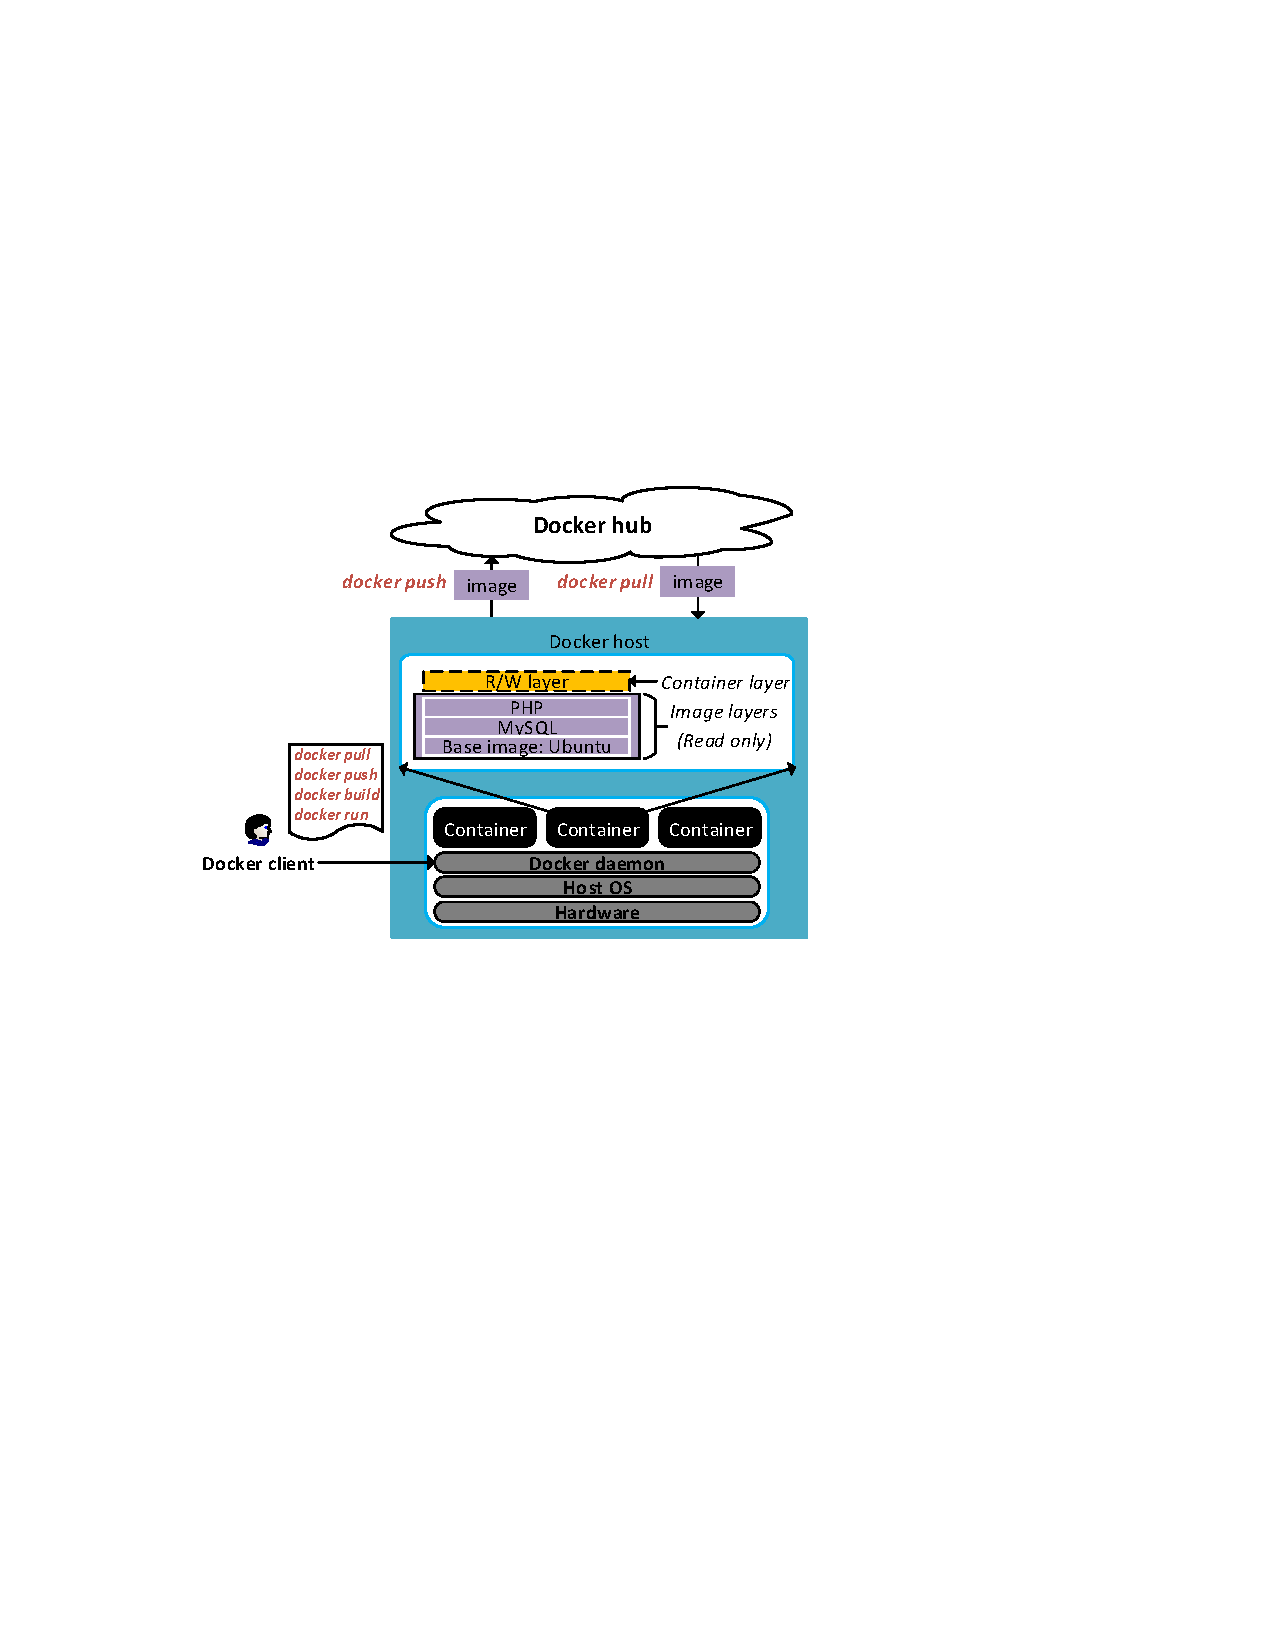
\includegraphics[width=0.5\textwidth]{graphs/fig-docker-architecture}
	\caption{Docker ecosystem
%	\lrcomment{We need to update the figure to capture
%	all the main interactions between the components and remove some unneeded
%	detail, \eg official and unofficial repositories\nancomment{addressed}}
	}
	\label{fig-docker-architecture}
\end{figure}
%
As shown in Figure~\ref{fig-docker-architecture}, a typical
Docker setup consists of three main components: \emph{client},
\emph{host}, and \emph{registry}.

Users interact with Docker using the Docker client which, in turn,
sends commands to the Docker host.
%
The client can be co-located on the host machine.
%
The Docker host runs a daemon process that implements the core logic of Docker and
is responsible for \emph{running} containers from locally available
images.
%
If a user tries to launch a container from an image that is not available
locally, the daemon \emph{pull}s the required image from the Docker registry.
%
Additionally, the daemon supports \emph{building} new images and \emph{pushing}
them to the registry.

\paragraph{Images and layers}
%
At the center of Docker is the concept of container images for packaging,
distributing, and running applications.
%
A Docker image consists of an ordered series of \emph{layers}.
%
Each Docker layer contains a subset of the files in the image and often represents a
specific component/dependency of the image, \eg a shared library.
%
Layers can be shared between two or more images if
the images depend on the same layer.
%
Image layers are read-only.
%
When users start a container, Docker creates a new
\emph{writable layer} on top of the underlying read-only layers
(Figure~\ref{fig-docker-architecture}).
%
Any changes made to files in the image will be reflected inside the writable
layer via a copy-on-write mechanism.
%%
%This leaves layers unmodified throughout the lifetime of a container and
%enables layer sharing across containers spawned from the same or different images.
%
%Docker supports multiple \emph{storage drivers} such as Aufs or Btrfs, which
%efficiently combine read-only and writable layers in a single
%namespace~\cite{docker-driver-eval}.
%
%The writable layers are deleted when the container is deleted.

%Image is represented by a \emph{manifest} which describes the various
%constituents of a Docker image, such as the target hardware platform and
%environment settings.
%%
%Moreover, the manifest contains a list of layer digests for all layers required
%by the image.


\paragraph{Registry}
%
The Docker registry is a platform for storing and distributing container images.
%
It stores images in \emph{repositories}, each containing different versions (\emph{tags}) of
the same image, identified as \texttt{<repo-name:tag>}.
%
For each image, the Docker registry stores a \emph{manifest} that describes,
among other things, which layers constitute the image.
%
%The manifest is a JSON file, which contains the runtime configuration for a
%container image (\eg target platform and environment variables) and the list
%of layers which make up the image.
%
Layers are identified via a digest that is computed as a hash (SHA-256)
over the uncompressed content of the layer and stored as compressed archival files.
%
%Image layers are stored as compressed archival files and image
%manifests as JSON files.
%
%\VT{What is image manifest? Need to introduce}
%
%
%Docker Hub is one of the most popular public registries, supporting both
%public and private repositories, via which users can upload, search, and
%download images~\cite{docker-hub}.
%
%In Docker Hub, the user repositories are namespaced by user name, i.e.,
%``$\langle username\rangle/\langle repository name \rangle$", while the
%official repositories, which are directly provided by Docker Inc. and partners
%are called ``$\langle repository name \rangle$".
%
%Modern Docker registry identifies and addresses a layer with a digest that is
%computed based on the uncompressed layer's content (e.g., SHA-256).
%
Identifying layers by their content allows the registry to store only one instance
of a layer even if it is referenced by multiple images.
%
%multiple users accidentally built identical layers.
%
%However, if at least one file differs in two otherwise identical layers,
%the two layers are treated as different and stored separately.
%


